% !TeX program = xelatex
\documentclass{beamer}
\usetheme{Madrid}
\usepackage{iftex}
\ifPDFTeX
  \usepackage[T5]{fontenc}
  \usepackage[utf8]{inputenc}
\else
  \usepackage{fontspec}
  \setsansfont{Inter}
\fi
\usepackage{booktabs}
\usepackage{array}
\usepackage{tikz}
\usetikzlibrary{positioning,shapes.geometric}
% Title slide
\title[E-Voucher System]{E-Voucher System -- Hệ thống bán voucher giảm giá trực tuyến}
\subtitle{Giới thiệu đồ án}
\author[Nhóm sinh viên]{Nguyễn Bình An, Lưu Ngô Quốc Bảo, Ngô Thế Đạt, Nguyễn Trọng Tín}
\institute[HCMUS]{Trường Đại học Khoa học Tự nhiên -- HCMUS}
\date{Tháng \the\month~năm \the\year}

\begin{document}

%--- Title page ---
\begin{frame}
  \titlepage
\end{frame}

%--- Thành viên ---
\begin{frame}{Thành viên dự án}
\begin{center}
\begin{tabular}{>{\bfseries}l l}
MSSV & Họ và tên \\
\midrule
23127149 & Nguyễn Bình An \\
23127327 & Lưu Ngô Quốc Bảo \\
23127340 & Ngô Thế Đạt (Nhóm trưởng) \\
23127498 & Nguyễn Trọng Tín \\
\end{tabular}
\end{center}
\end{frame}

%--- Vai trò trong hệ thống ---
\begin{frame}{Các vai trò trong hệ thống}
\begin{itemize}
  \item \textbf{Khách hàng}: Người dùng cuối mua và nhận voucher.
  \item \textbf{Đối tác}: Doanh nghiệp phát hành voucher.
  \item \textbf{Nhân viên đối tác}: Nhân viên của đối tác thực hiện bán/vận hành voucher.
  \item \textbf{Quản trị viên (Admin)}: Quản lý tài khoản, đối tác, voucher, đơn hàng, báo cáo.
\end{itemize}
\end{frame}

%--- Kiến trúc tổng quan ---
\begin{frame}{Kiến trúc tổng quan}
\begin{figure}
  \centering
  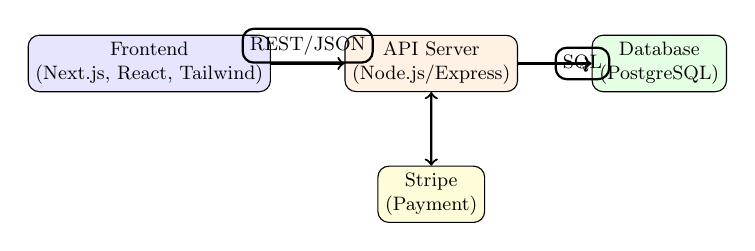
\begin{tikzpicture}[
    scale=0.78,
    transform shape,
    node distance=1.2cm and 1.2cm,
    every node/.style={draw,rounded corners,align=center,font=\small}
  ]
    \node[fill=blue!10] (frontend) {Frontend\\(Next.js, React, Tailwind)};
    \node[right=of frontend, fill=orange!10] (api) {API Server\\(Node.js/Express)};
    \node[right=of api, fill=green!10] (db) {Database\\(PostgreSQL)};
    \node[below=of api, fill=yellow!15] (stripe) {Stripe\\(Payment)};
    \draw[->, thick] (frontend) -- (api) node[midway,above] {REST/JSON};
    \draw[->, thick] (api) -- (db) node[midway,right] {SQL};
    \draw[<->, thick] (api) -- (stripe);
  \end{tikzpicture}
  \caption{Kiến trúc 3 lớp: Frontend -- API -- Database}
\end{figure}
\end{frame}

%--- Use-case diagram ---
\begin{frame}{Use-case diagram}
\centering
\begin{tikzpicture}[
  actor/.style={draw,rounded corners,fill=blue!10,minimum width=2.2cm,minimum height=0.8cm},
  usecase/.style={draw,ellipse,fill=green!10,minimum width=3.1cm,minimum height=0.75cm},
  every node/.append style={align=center,font=\small}
]
  \node[actor] (customer) at (-4,1.5) {Khách hàng};
  \node[actor] (partner) at (-4,-1.5) {Đối tác};
  \node[actor] (admin) at (4,0) {Quản trị viên};
  \node[usecase] (browse) at (0,2) {Tìm kiếm voucher};
  \node[usecase] (purchase) at (0,0.7) {Mua và thanh toán};
  \node[usecase] (manage) at (0,-0.7) {Quản lý voucher};
  \node[usecase] (report) at (0,-2) {Quản lý và báo cáo};
  \draw (customer) -- (browse);
  \draw (customer) -- (purchase);
  \draw (partner) -- (manage);
  \draw (admin) -- (manage);
  \draw (admin) -- (report);
\end{tikzpicture}

\vspace{0.4em}
{\tiny Biểu đồ khái quát các ca sử dụng chính của hệ thống.}
\end{frame}

%--- Công nghệ và stack ---
\begin{frame}{Công nghệ \& Stack}
\begin{columns}
  \column{0.5\textwidth}
  \textbf{Frontend}
  \begin{itemize}
    \item Next.js 16 (React 18)
    \item Tailwind CSS 3
    \item lucide-react, sonner, clsx
    \item @dnd-kit/react (drag-drop)
    \item qrcode.react, @zxing/browser (QR/Barcode)
  \end{itemize}
  \column{0.5\textwidth}
  \textbf{Backend}
  \begin{itemize}
    \item Node.js (TypeScript)
    \item Express 5
    \item PostgreSQL
    \item Stripe (payment gateway)
    \item AWS S3 SDK, Nodemailer
    \item Security: cors, helmet, express-rate-limit
  \end{itemize}
\end{columns}
\end{frame}

%--- Hình thức thanh toán ---
\begin{frame}{Hình thức thanh toán}
\begin{itemize}
  \item Thanh toán qua \textbf{Stripe} (thẻ Visa/MasterCard, ví điện tử).
  \item Quy trình: Chọn phương thức $\rightarrow$ Xác nhận $\rightarrow$ Cập nhật trạng thái (paid / failed / refunded).
  \item Ghi lại chi tiết giao dịch trong bảng \texttt{orders}.
\end{itemize}
\end{frame}

%--- Thông tin hosting / VPS ---
\begin{frame}{Môi trường triển khai (Hosting / VPS)}
\begin{itemize}
  \item Frontend được build bởi \texttt{next build} và phục vụ dưới dạng static assets.
  \item Backend chạy dưới Node.js (PM2 hoặc Docker) trên VPS/Linux.
  \item Cơ sở dữ liệu PostgreSQL host trên VPS hoặc dịch vụ quản lý (RDS, DigitalOcean Managed DB).
  \item SSL/TLS được cấu hình qua reverse proxy (nginx) hoặc nền tảng cloud.
\end{itemize}
\end{frame}

%--- Kết luận và hướng phát triển ---
\begin{frame}{Kết luận \& Hướng phát triển}
\begin{itemize}
  \item Hoàn thành hệ thống bán voucher end-to-end với quản trị đa vai trò.
  \item Đã triển khai các tính năng chính: đăng ký, tìm kiếm, mua, thanh toán, quản lý voucher.
  \item \textbf{Hướng mở rộng}:
    \begin{itemize}
      \item Tích hợp thêm các phương thức thanh toán (MoMo, ZaloPay).
      \item Mobile app (React Native) cho khách hàng.
      \item Báo cáo BI với Power BI hoặc Metabase.
    \end{itemize}
\end{itemize}
\end{frame}

\end{document}
